%% Hawkeye — CIKM 2026 submission draft.
%% Compiles on Overleaf with the ACM "acmart" class (sigconf). "nonacm" drops
%% the copyright boilerplate for a clean draft; remove "review" for camera-ready.
\documentclass[sigconf,nonacm,review]{acmart}
\settopmatter{printacmref=false}
\pagestyle{plain}

\usepackage{graphicx}
\usepackage{booktabs}
\usepackage{amsmath}
\usepackage{xcolor}
\usepackage{multirow}
\usepackage{array}
\usepackage{xspace}
\usepackage{tikz}
\usetikzlibrary{arrows.meta,positioning,calc,fit,backgrounds}

\newcommand{\todo}[1]{\textcolor{red}{[TODO: #1]}}
\newcommand{\tbd}{\textcolor{red}{\textit{TBD}}}
\newcommand{\method}{\textsc{Hawkeye}\xspace}
\newcommand{\R}{\mathbb{R}}
\newcommand{\Ncal}{\mathcal{N}}
\newcommand{\Ecal}{\mathcal{E}}
\newcommand{\Gcal}{\mathcal{G}}
\newcommand{\Vcal}{\mathcal{V}}

\begin{document}

\title{Hawkeye: Seeing One Layer Deeper --- A Cohesion-Aware Structural Channel
for Temporal Link Prediction}

%% ---- DOUBLE-BLIND: anonymised for submission. ----
%% Camera-ready authors (do NOT uncomment for the review submission):
%%   Jiacheng Ding  <jding2@memphis.edu>
%%   Xiaofei Zhang  <xiaofei.zhang@memphis.edu>
%%   The University of Memphis
\author{Anonymous Author(s)}
\affiliation{\institution{Anonymous Institution}\country{}}
\email{anonymous@example.com}

\renewcommand{\shortauthors}{Anonymous}
\hypersetup{pdfauthor={}}

\begin{abstract}
State-of-the-art temporal-link-prediction (TLP) models are, in essence,
multi-channel information aggregators: they combine an interaction-history
channel, a time-encoding channel, and a \emph{structure channel}. The first two
have been refined relentlessly; the structure channel remains a crude
afterthought --- DyGFormer encodes it as a $1$--$2$-bit neighbour-cooccurrence
count. We begin with a measurement: on sparse temporal graphs the classical
$1$-hop common-neighbour signal is near-random (discriminative AUC
$\approx 0.50$), because two nodes almost never share a direct neighbour; the
genuinely discriminative signal lies one hop deeper --- the \emph{2-hop cohesive
bridge}, whose discAUC reaches $0.74$--$0.96$, on both bipartite and
non-bipartite graphs. Motivated by this, we propose \method, a cohesion-aware
structural channel that incrementally maintains the classical $k$-family of
cohesiveness indicators (degree $\to$ $k$-core $\to$ $k$-truss) and forms
2-hop cohesive-bridge features. \method is a drop-in replacement for a
temporal-graph model's native structure channel, with no change to the
backbone. Swapping \method into DyGFormer raises test MRR on
\texttt{tgbl-wiki} from $0.779$ to $0.807$ and test AP on \texttt{CanParl} from
$0.700$ to $0.740$. We further characterise \emph{when} it helps: the gain
tracks a graph's structural diversity and vanishes on near-complete graphs ---
a predictable boundary. All code, data and figure scripts are released.
\end{abstract}

\keywords{temporal link prediction, dynamic graphs, $k$-core, $k$-truss,
structural features, graph neural networks}

\maketitle

%% ===================================================================
\section{Introduction}
\label{sec:intro}

Many real-world systems are naturally represented as graphs that \emph{evolve
over time}: user interactions in social networks~\cite{trivedi2019dyrep},
user--item engagements on e-commerce and streaming
platforms~\cite{kumar2019jodie}, account-to-account transactions in financial
systems~\cite{huang2023tgb}, the evolution of entity relations in knowledge
graphs, and device connections in communication networks. Forecasting which new
edges will appear next on such evolving graphs --- \emph{temporal link
prediction} (TLP) --- is a fundamental and practically important task: it
underpins friend recommendation, fraud and anti-money-laundering detection, and
drug--target discovery~\cite{poursafaei2022edgebank,huang2023tgb}.

Temporal-graph learning has advanced rapidly, and the prevailing paradigm
models the \emph{interaction dynamics} of nodes. TGN maintains a per-node
\emph{memory} module updated by every interaction event~\cite{rossi2020tgn}.
DyGFormer feeds the chronologically ordered sequence of a node's historical
neighbours into a Transformer~\cite{yu2023dygformer}. TPNet builds and projects
a temporal random-walk matrix and reaches state-of-the-art accuracy without a
GNN architecture~\cite{lu2024tpnet}. TNCN dynamically maintains a neighbour
dictionary and strengthens pairwise representations with temporal
common-neighbour signals~\cite{zhang2024tncn}; very recent work further refines
interaction-pattern awareness and causal
debiasing~\cite{zhang2025ipnet,zhang2025tide}. Earlier attention-, walk- and
mixing-based encoders share the same
spirit~\cite{xu2020tgat,wang2021cawn,cong2023graphmixer}. These methods differ
in emphasis but share one core idea: encode the interaction-history sequence
--- \emph{who interacted with whom, and when} --- and score candidate edges
from the learned embeddings.

Architecturally, a state-of-the-art temporal-graph model is a
\emph{multi-channel information aggregator}: (a) an interaction-history channel,
(b) a time-encoding channel, and (c) a \emph{structure channel} encoding the
topological relation between the candidate pair. The first two channels have
been refined relentlessly --- from RNNs to Transformers to state-space models
--- yet the structure channel remains a \emph{crude afterthought}. DyGFormer's
structure channel is merely a $1$--$2$-bit neighbour-cooccurrence count; TNCN's
is a single common-neighbour count. Behind these designs lies an unstated
assumption: that the \textbf{1-hop common neighbour} is the right structural
signal. Is it?

A systematic measurement study says it is not. Streaming each benchmark
chronologically and scoring every candidate structural feature by how well it
separates true edges from the official negatives, we find that \textbf{on
sparse temporal graphs the 1-hop common-neighbour signal is barely better than
a coin flip}: discriminative AUC $\approx 0.50$ on \texttt{tgbl-uci},
\texttt{tgbl-enron} and \texttt{tgbl-wiki}. These graphs are too sparse for two
arbitrary nodes to share a \emph{direct} neighbour. The genuinely
discriminative signal lies \emph{one hop deeper} --- the \textbf{2-hop cohesive
bridge}: whether two nodes are embedded in the same densely connected region
through length-2 paths. Its discAUC reaches $0.74$--$0.96$, and this holds on
\emph{both} bipartite and non-bipartite graphs --- the deciding factor is
sparsity, not graph type.

\begin{figure}[t]
\centering
% Figure 1 — Running example threaded through the paper.
% Corporate-email setting. Alice (u) and Bob (v) have never emailed
% (CN=0). Two convex 2-hop cohesive bridges connect them: an upper
% high-cohesion bridge Carol--Dan and a lower bridge Eve--Grace.
% Per Def 6, bridge_c sums core numbers over BOB's neighbours in
% N_2(Alice), i.e. c(Dan) + c(Grace).
%
% Hand-drawn-feel: asymmetric vertical offsets between the two
% bridges, asymmetric horizontal spans, every edge audited.
% Labels are placed OUTSIDE the figure perimeter so they never
% overlap any edge.
%
% EDGE AUDIT (every edge below):
%   Alice--Carol   solid  gray   real 1-hop edge
%   Alice--Eve     solid  gray   real 1-hop edge
%   Alice--Hank    solid  gray   real 1-hop edge (degree asymmetry)
%   Bob--Dan       solid  gray   real 1-hop edge
%   Bob--Grace     solid  gray   real 1-hop edge
%   Carol--Dan     solid  ORANGE real edge, highlighted as upper 2-hop bridge
%   Eve--Grace     solid  ORANGE real edge, highlighted as lower 2-hop bridge
%   Alice--Bob     DASHED gray   candidate future edge (does not yet exist)
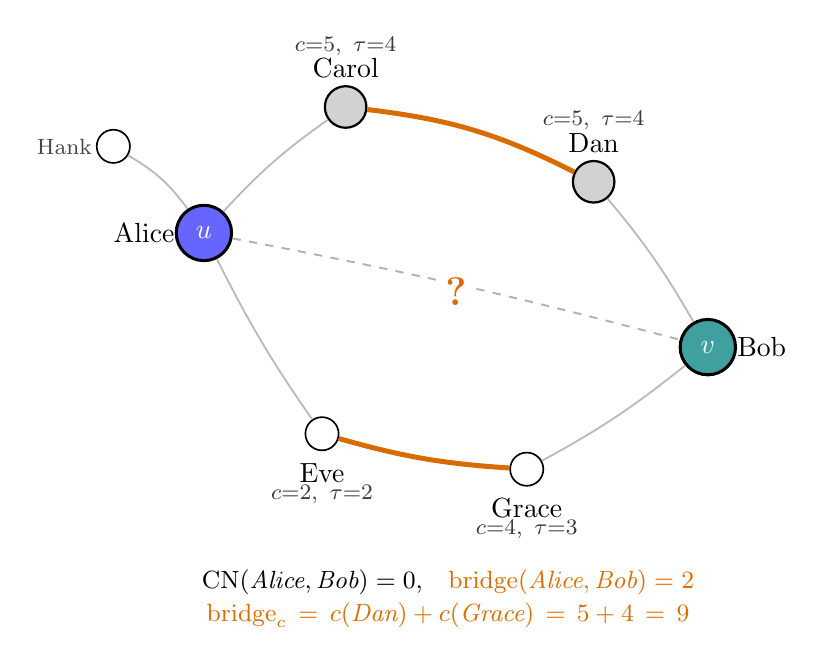
\begin{tikzpicture}[
  every node/.style={font=\rmfamily\normalsize},
  nd/.style={circle,draw,minimum size=12pt,inner sep=0pt,fill=white,
             line width=0.6pt},
  hi/.style={circle,draw,minimum size=15pt,inner sep=0pt,fill=gray!35,
             line width=0.8pt},
  qry/.style={circle,draw,minimum size=20pt,inner sep=0pt,
              line width=1.1pt},
  brg/.style={orange!85!black,line width=1.8pt},
  ed/.style ={gray!55,line width=0.65pt},
  cq/.style ={font=\rmfamily\footnotesize,gray!45!black},
  x=1cm,y=1cm]

  % --- Query nodes: Alice high-left, Bob low-right; intentional tilt
  \node[qry,fill=blue!60,text=white] (u) at (-0.40, 1.85) {$u$};
    \node[anchor=east] at (-0.65, 1.85) {Alice};
  \node[qry,fill=teal!75,text=white] (v) at ( 6.00, 0.40) {$v$};
    \node[anchor=west] at ( 6.25, 0.40) {Bob};

  % --- UPPER bridge nodes (high cohesion). Carol and Dan are NOT at the same y
  \node[hi] (carol) at (1.40, 3.45) {};
    \node[anchor=south] at (1.40, 3.70) {Carol};
    \node[cq,anchor=south] at (1.40, 3.98) {$c{=}5,\ \tau{=}4$};
  \node[hi] (dan)   at (4.55, 2.50) {};
    \node[anchor=south] at (4.55, 2.75) {Dan};
    \node[cq,anchor=south] at (4.55, 3.03) {$c{=}5,\ \tau{=}4$};

  % --- LOWER bridge nodes. Lower bridge is INTENTIONALLY shorter in x-span
  %     and shifted left, so the figure is not a y-mirror.
  \node[nd] (eve)   at (1.10,-0.70) {};
    \node[anchor=north] at (1.10,-0.95) {Eve};
    \node[cq,anchor=north] at (1.10,-1.23) {$c{=}2,\ \tau{=}2$};
  \node[nd] (grace) at (3.70,-1.15) {};
    \node[anchor=north] at (3.70,-1.40) {Grace};
    \node[cq,anchor=north] at (3.70,-1.68) {$c{=}4,\ \tau{=}3$};

  % --- Alice's extra non-bridge contact. We name him "Hank" so the small
  %     circle isn't a stray dot; he's an Alice-only contact who plays no
  %     role in the (Alice, Bob) bridge story.
  \node[nd] (hank) at (-1.55, 2.95) {};
    \node[font=\rmfamily\footnotesize,gray!55!black,anchor=east] at (-1.70, 2.95) {Hank};

  % --- EDGES (audited above) ---
  % Alice's 1-hop edges (real, solid gray)
  \draw[ed] (u) to[bend left=6]   (carol);     % Alice -- Carol
  \draw[ed] (u) to[bend right=4]  (eve);       % Alice -- Eve
  \draw[ed] (u) to[bend right=12] (hank);      % Alice -- Hank (curvier to avoid the "stray dot" look)
  % Bob's 1-hop edges (real, solid gray)
  \draw[ed] (v) to[bend right=5]  (dan);       % Bob   -- Dan
  \draw[ed] (v) to[bend left=5]   (grace);     % Bob   -- Grace
  % The two 2-hop cohesive bridges (real edges, highlighted orange thick)
  \draw[brg] (carol) to[bend left=10] (dan);   % Carol -- Dan   upper bridge
  \draw[brg] (eve)   to[bend right=6] (grace); % Eve   -- Grace lower bridge
  % Candidate future edge: dashed (does not yet exist)
  \draw[dashed,gray!60,line width=0.7pt] (u) to[bend left=2] (v);

  % --- "?" in the central clear space. Bumped color + size + behind a tiny
  %     white halo so it reads even where it crosses the faint dashed Alice-Bob
  %     edge.
  \node[fill=white,inner sep=1pt,
        font=\rmfamily\Large\bfseries,text=orange!85!black] at (2.80, 1.10) {?};

  % --- bottom annotation: the formula the figure illustrates
  \node[font=\rmfamily\small,anchor=north,align=center]
       at (2.70,-2.30)
    {$\mathrm{CN}(\textit{Alice},\textit{Bob})=0$,\quad
     \textcolor{orange!85!black}{$\mathrm{bridge}(\textit{Alice},\textit{Bob})=2$}\\[1pt]
     \textcolor{orange!85!black}{$\mathrm{bridge}_c\,=\,c(\textit{Dan})+c(\textit{Grace})\,=\,5+4\,=\,9$}};
\end{tikzpicture}

\caption{Running example. Nodes $u$ and $v$ share no 1-hop common neighbour
($\mathrm{CN}=0$), so a cooccurrence-based structure channel sees no signal.
Yet $u$ and $v$ are joined by two \emph{2-hop cohesive bridges} through
high-coreness intermediaries ($a,d$ with core $5,4$), revealing that the pair
is embedded in the same dense structural region.}
\label{fig:running}
\end{figure}

Motivated by this finding, we propose \method, a \emph{cohesion-aware structure
channel} that lets a temporal-graph model ``see one layer deeper''
(Figure~\ref{fig:running}). \method
incrementally maintains, over the edge stream, the classical $k$-family of
structural-cohesiveness indicators --- degree $\to$ $k$-core $\to$ $k$-truss ---
and forms \textbf{2-hop cohesive-bridge} pairwise features. It is a
\textbf{drop-in replacement} for a temporal-graph model's native structure
channel: it changes \emph{what} structural signal the backbone receives without
changing the backbone. Swapping \method into DyGFormer raises test MRR on
\texttt{tgbl-wiki} from $0.779$ to $0.807$ (above the reported DyGFormer
result) and test AP on \texttt{CanParl} from $0.700$ to $0.740$. We further
\emph{characterise when it helps}: the gain tracks a graph's structural
diversity; on near-complete graphs every node attains the same maximal coreness
and \method correctly does not help --- a predictable boundary.

\paragraph{Contributions.}
(1) An empirical finding: 1-hop common neighbours are near-random on sparse
temporal graphs (discAUC $\approx 0.50$); the \textbf{2-hop cohesive bridge} is
the dominant simple structural signal (discAUC $0.74$--$0.96$), on bipartite
and non-bipartite graphs alike.
(2) \method: an incrementally maintained, cohesion-aware structure channel
built on the $k$-family, which plug-and-play replaces the native structure
channel of any temporal-graph backbone.
(3) A characterisation of \emph{when} structural augmentation helps --- the
gain is predicted by a training-free structural-diversity measure.
(4) Experiments across TGB and DGB datasets: $+2.8$--$4$ points over SOTA
DyGFormer on non-degenerate graphs, with honest boundary results on degenerate
graphs.

%% ===================================================================
\section{Preliminary}
\label{sec:prelim}

\subsection{Problem Formulation}
A \emph{continuous-time dynamic graph} is a time-ordered stream of edges
\begin{equation}
\Gcal = \{(u_1,v_1,t_1),\dots,(u_m,v_m,t_m)\},\quad t_1\le\dots\le t_m,
\end{equation}
with nodes $u_i,v_i\in\Vcal$ and timestamps $t_i\in\R^{+}$. The cumulative
snapshot $\Gcal(t)$ is the simple undirected graph induced by all edges with
timestamp $\le t$; $\Gcal(<t)$ denotes the strictly-earlier history. Given
$\Gcal(<t)$, a query node $u$, and candidate destinations $\mathcal{C}$,
\emph{temporal link prediction} assigns a score $s(u,v,t)$ to each
$v\in\mathcal{C}$ so the truly-occurring edge is ranked highest:
\begin{equation}
v^{*}=\arg\max_{v\in\mathcal{C}} s(u,v,t).
\end{equation}
Following TGB~\cite{huang2023tgb}, accuracy is the mean reciprocal rank (MRR);
on DGB datasets~\cite{poursafaei2022edgebank} we report average precision (AP).

\subsection{The $k$-family of Cohesiveness Indicators}
\method measures how densely a node is embedded via the classical $k$-family.
A subgraph $H$ is a \emph{$k$-core} iff every node in $H$ has degree $\ge k$
within $H$ and $H$ is maximal; the \emph{core number} is
\begin{equation}
c(v)=\max\{k:v\in k\text{-core}(\Gcal(t))\}.
\end{equation}
A subgraph $H$ is a \emph{$k$-truss} iff every edge of $H$ is supported by
$\ge k-2$ triangles within $H$; the \emph{trussness} is
\begin{equation}
\tau(v)=\max\{k:\exists\,(v,w)\in k\text{-truss}(\Gcal(t))\}.
\end{equation}
The family is nested,
\begin{equation}
k\text{-truss}\subseteq(k-1)\text{-core},
\end{equation}
forming a loose-to-tight spectrum degree $\to$ $k$-core $\to$ $k$-truss
\cite{seidman1983kcore,batagelj2003cores,cohen2008trusses,wang2012truss}. A
tighter constraint describes finer structure but costs more to maintain:
$O(1)$ per edge for degree, $O(\text{local})$ for $k$-core, up to $O(m^{1.5})$
for $k$-truss. Intuitively, the three ask increasingly strict questions:
``do you have neighbours?'' / ``do your neighbours have enough neighbours?'' /
``do your neighbours know each other?''

\subsection{The 2-hop Cohesive Bridge}
The 2-hop neighbourhood of $u$ is
$\Ncal_2(u,t)=\{w:\exists z,\,(u,z),(z,w)\in\Gcal(t),\,w\neq u\}$. For a
candidate pair $(u,v)$, the \emph{2-hop cohesive-bridge} strength is
\begin{equation}
\mathrm{bridge}(u,v,t)=\bigl|\{w\in\Ncal(v,t):w\in\Ncal_2(u,t)\}\bigr|,
\end{equation}
the number of $v$'s direct neighbours reachable from $u$ in two hops. Even when
$u,v$ share no direct neighbour, a large bridge means they are embedded in the
same structural community. A cohesion-weighted variant
$\mathrm{bridge}_c(u,v,t)=\sum_{w}c(w)$ up-weights bridges through highly
cohesive intermediaries. The classical 1-hop count
$\mathrm{CN}(u,v,t)=|\Ncal(u,t)\cap\Ncal(v,t)|$ is strong for static link
prediction~\cite{liben2007linkpred} but, as shown next, near-random on sparse
temporal graphs.

%% ===================================================================
\section{Empirical Study: Why Existing Structural Signals Fail}
\label{sec:study}

Before presenting the method, we use \emph{training-free measurement} to
characterise the structural signal. On six TGB datasets we stream each
benchmark chronologically and, for every validation edge and its negatives,
compute each candidate structural feature on $\Gcal(<t)$, reporting its
\emph{discriminability AUC} (discAUC): the probability it ranks the true edge
above a negative. discAUC $=0.50$ is random.

\paragraph{F1: 1-hop CN is near-random on sparse graphs; 2-hop is the signal.}
Table~\ref{tab:discauc} reports the discAUC of the 1-hop common neighbour and
the 2-hop cohesive bridge. On \texttt{tgbl-uci}, \texttt{tgbl-enron} and
\texttt{tgbl-wiki} the 1-hop CN has discAUC $=0.50$ --- it cannot distinguish a
true edge from a negative, because these graphs are too sparse for two nodes to
share a direct neighbour. The 2-hop cohesive bridge, on the same datasets,
reaches $0.73$--$0.96$. This is not a bipartite artefact: \texttt{tgbl-uci} and
\texttt{tgbl-enron} are non-bipartite, yet their 1-hop CN is equally random ---
the factor that decides whether 1-hop CN works is graph \emph{sparsity}. On the
denser \texttt{tgbl-coin}, 1-hop CN already works ($0.75$); and on the
degenerate near-complete \texttt{tgbl-lastfm} even the 2-hop bridge is
near-random ($0.53$), foreshadowing \method's boundary
(\S\ref{sec:exp}).

\begin{table}[t]
\caption{Discriminability AUC of 1-hop vs.\ 2-hop structural signals
(discAUC $=0.50$ is random). 1-hop CN is random on sparse graphs; the 2-hop
cohesive bridge is strongly discriminative.}
\label{tab:discauc}
\centering\small
\setlength{\tabcolsep}{4pt}
\begin{tabular}{llccc}
\toprule
dataset & density & 1-hop & 2-hop & 2-hop$\times$c \\
\midrule
\texttt{tgbl-uci}       & sparse           & 0.50 & \textbf{0.76} & 0.75 \\
\texttt{tgbl-enron}     & sparse           & 0.50 & \textbf{0.73} & 0.71 \\
\texttt{tgbl-wiki}      & sparse           & 0.50 & \textbf{0.85} & 0.83 \\
\texttt{tgbl-subreddit} & medium           & 0.50 & \textbf{0.96} & 0.96 \\
\texttt{tgbl-coin}      & denser           & 0.75 & 0.77 & 0.77 \\
\texttt{tgbl-lastfm}    & degen.-dense     & 0.50 & 0.53 & 0.52 \\
\bottomrule
\end{tabular}
\\[2pt]
{\footnotesize 1-hop = common neighbour; 2-hop = cohesive bridge;
2-hop$\times$c = core-weighted.}
\end{table}

\begin{figure}[t]
\centering

\includegraphics[width=0.92\columnwidth]{figures/fig_discauc.pdf}
\caption{Discriminability AUC of 1-hop common neighbours vs.\ 2-hop cohesive
bridges across six temporal-graph benchmarks. On sparse graphs the 1-hop CN is
no better than random ($0.50$); 2-hop bridges reach discAUC $0.73$--$0.96$.}
\label{fig:discauc}
\end{figure}

\paragraph{F2: $k$-family weighting $\approx$ raw 2-hop count.}
The last two columns of Table~\ref{tab:discauc} show that core-weighting the
2-hop bridge barely changes its discAUC ($0.76$ vs.\ $0.75$ on uci). We report
this honestly: the 2-hop \emph{topology} is the dominant signal; $k$-family
weighting is a refinement, not the driver. The value of the $k$-family is
twofold --- as node-level features and as the incrementally maintained
substrate on which the 2-hop bridge is computed.

\paragraph{F3: the constraint hierarchy degree $\to$ core $\to$ truss.}
In a struct-only setting (no GNN), the predictive power of the $k$-family
increases monotonically with constraint tightness: on \texttt{tgbl-uci} the
validation MRR is degree $0.022\to$ $k$-core $0.030\to$ $k$-truss $0.097$.
A tighter constraint yields a finer signal, but $k$-truss costs far more to
maintain. \textbf{$k$-core is the efficiency--effectiveness sweet spot}, and is
\method's default indicator.

%% ===================================================================
\section{Method: Hawkeye}
\label{sec:method}

\method is a \emph{structure-channel replacement module}: it does not modify
the backbone --- it replaces only the backbone's native structure channel. We
instantiate it on DyGFormer~\cite{yu2023dygformer}, swapping out the
neighbour-cooccurrence encoder. \method has three components (Figure~\ref{fig:arch}):
(A) a \emph{Cohesion Cache} maintaining the $k$-family and graph adjacency over
the stream; (B) \emph{Pairwise Feature Extraction} computing 2-hop
cohesive-bridge features; (C) a \emph{Cohesion Slot Encoder} projecting those
features into the per-slot embedding fed to the Transformer.

\begin{figure}[t]
\centering
% Figure 3 — Per-batch timing of Hawkeye, threaded with the Alice/Bob
% running example. Layout is a CLOCKWISE LOOP that uses the
% predict-then-advance feedback as structural backbone — this keeps the
% overall aspect ratio close to 2.2:1 rather than a long thin strip.
%
% Reading order: top row (CPU lane, INPUT -> P1 .. P4) -> right column
% (P5 -> P6+P7 on GPU) -> bottom row (OUTPUT -> P8 advance cache via the
% predict-then-advance arrow) -> left column (P8 -> INPUT for next batch).
%
% The orange P1..P8 step badges of the previous version are gone; each
% step's number is inline at the start of its block ("P1. ...").
%
% Alice/Bob are present at INPUT, P3, P4, GPU, OUTPUT, P8 — every box
% the running example actually touches.
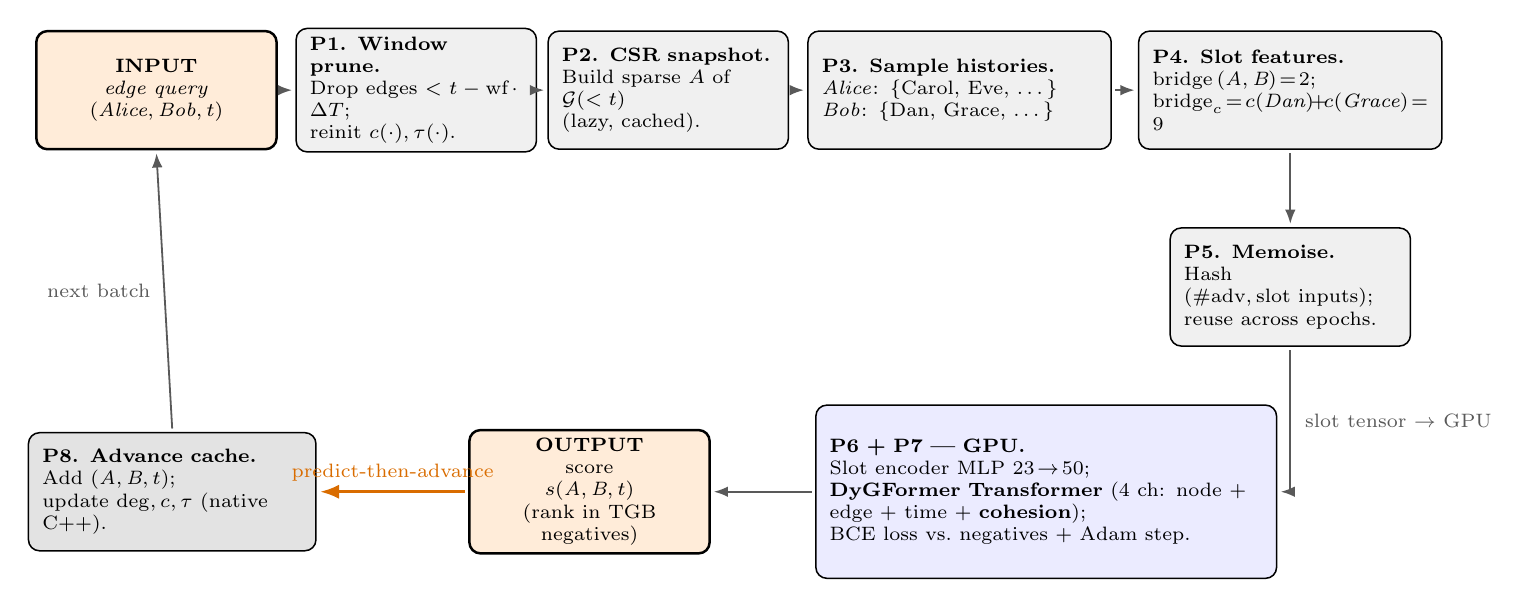
\begin{tikzpicture}[
  every node/.style={font=\rmfamily\scriptsize},
  cstep/.style ={rounded corners,draw,align=left,inner xsep=5pt,inner ysep=3pt,
                outer sep=1.5pt,
                fill=gray!12,line width=0.55pt,
                text width=27mm,minimum height=15mm},
  cstepw/.style={rounded corners,draw,align=left,inner xsep=5pt,inner ysep=3pt,
                outer sep=1.5pt,
                fill=gray!12,line width=0.55pt,
                text width=35mm,minimum height=15mm},
  gpu/.style  ={rounded corners,draw,align=left,inner xsep=5pt,inner ysep=3pt,
                outer sep=1.5pt,
                fill=blue!8,line width=0.55pt,
                text width=55mm,minimum height=22mm},
  endpt/.style={rounded corners,draw,align=center,inner xsep=5pt,inner ysep=3pt,
                outer sep=1.5pt,
                fill=orange!15,line width=0.9pt,
                text width=27mm,minimum height=15mm},
  cache/.style={rounded corners,draw,align=left,inner xsep=5pt,inner ysep=3pt,
                outer sep=1.5pt,
                fill=gray!22,line width=0.55pt,
                text width=33mm,minimum height=15mm},
  fl/.style   ={-{Latex[length=1.8mm]},line width=0.65pt,gray!70!black},
  fb/.style   ={-{Latex[length=2.4mm]},line width=1.0pt,orange!85!black},
  x=1mm,y=1mm]

  % ===== TOP ROW (CPU lane): INPUT -> P1 -> P2 -> P3 -> P4 =====
  % Each pair of adjacent boxes has ~6mm of clear space between borders.
  \node[endpt] (inp) at ( 15, 75)
    {\textbf{INPUT}\\\textit{edge query}\\$(\textit{Alice},\textit{Bob},t)$};
  \node[cstep]  (p1)  at ( 48, 75)
    {\textbf{P1. Window prune.}\\Drop edges $<t-\mathrm{wf}\!\cdot\!\Delta T$;\\reinit $c(\cdot),\tau(\cdot)$.};
  \node[cstep]  (p2)  at ( 80, 75)
    {\textbf{P2. CSR snapshot.}\\Build sparse $A$ of $\Gcal(<t)$\\(lazy, cached).};
  \node[cstepw] (p3)  at (117, 75)
    {\textbf{P3. Sample histories.}\\\textit{Alice}: \{Carol, Eve, \ldots\}\\\textit{Bob}: \{Dan, Grace, \ldots\}};
  \node[cstepw] (p4)  at (159, 75)
    {\textbf{P4. Slot features.}\\$\mathrm{bridge}\,(\textit{A},\textit{B})\!=\!2$;\\
     $\mathrm{bridge}_c\!=\!c(\textit{Dan})\!+\!c(\textit{Grace})\!=\!9$};

  % ===== RIGHT COLUMN: P5 -> GPU (CPU/GPU handoff) =====
  \node[cstep]  (p5)  at (159, 50)
    {\textbf{P5. Memoise.}\\Hash $(\#\text{adv}, \text{slot inputs})$;\\reuse across epochs.};
  \node[gpu]   (gpu) at (128, 24)
    {\textbf{P6 + P7 — GPU.}\\Slot encoder MLP $23\!\to\!50$;\\
     \textbf{DyGFormer Transformer} (4 ch: node $+$ edge $+$ time $+$ \textbf{cohesion});\\
     BCE loss vs.\ negatives $+$ Adam step.};

  % ===== BOTTOM ROW (returns LEFT): OUTPUT -> P8 =====
  \node[endpt] (out) at ( 70, 24)
    {\textbf{OUTPUT}\\score \\$s(\textit{A},\textit{B},t)$\\(rank in TGB negatives)};
  \node[cache] (p8)  at ( 17, 24)
    {\textbf{P8. Advance cache.}\\Add $(\textit{A},\textit{B},t)$;\\update $\deg, c, \tau$ (native C++).};

  % ===== ARROWS =====
  % CPU top row: left to right
  \draw[fl] (inp.east) -- (p1.west);
  \draw[fl] (p1.east)  -- (p2.west);
  \draw[fl] (p2.east)  -- (p3.west);
  \draw[fl] (p3.east)  -- (p4.west);
  % Right column down (CPU -> GPU handoff has its own label).
  % p5 -> gpu is a bent "down-then-left" path so the label sits in clean space.
  \draw[fl] (p4.south) -- (p5.north);
  \draw[fl] (p5.south) |- node[pos=0.25,right,font=\rmfamily\scriptsize,xshift=0.6mm]
                              {slot tensor $\to$ GPU} (gpu.east);
  % GPU produces OUTPUT (going left along bottom row)
  \draw[fl] (gpu.west) -- (out.east);
  % predict-then-advance feedback (orange) — OUTPUT -> P8
  \draw[fb] (out.west) -- node[above,font=\rmfamily\scriptsize]
                              {predict-then-advance} (p8.east);
  % Loopback: P8 -> INPUT (next batch)
  \draw[fl] (p8.north) -- node[left,font=\rmfamily\scriptsize,xshift=-0.5mm]
                              {next batch} (inp.south);

\end{tikzpicture}

\caption{\method as a drop-in structure channel for DyGFormer. The Cohesion
Cache (A) incrementally maintains $k$-family indicators on CPU; Pairwise
Feature Extraction (B) computes 2-hop cohesive-bridge features; the Cohesion
Slot Encoder (C) projects them into the per-slot embedding that replaces
DyGFormer's native cooccurrence channel. The Transformer backbone (dashed) is
unchanged.}
\label{fig:arch}
\end{figure}

\subsection{Cohesion Cache: Incremental Structural Maintenance}
The Cohesion Cache maintains, as edges arrive, (a) a CSR-backed adjacency
structure and (b) per-node $k$-family indicators. On edge $(u,v,t)$ the degree
update is
\begin{equation}
d(u)\leftarrow d(u)+1,\qquad d(v)\leftarrow d(v)+1,
\end{equation}
at $O(1)$ cost. The core-number update is local: with $k=\min(c(u),c(v))$, only
nodes near the core frontier can change, and the affected set $S$ is promoted,
\begin{equation}
c(w)\leftarrow c(w)+1\quad\text{for }w\in S,
\end{equation}
following streaming $k$-core
maintenance~\cite{batagelj2003cores,sariyuce2013kcorestream}; $|S|\ll|\Vcal|$ in
practice, so the update is millisecond-scale. Trussness is maintained
analogously at higher cost; degree$+$core is the efficient default. Optionally,
a sliding window of size $W$ evicts edges older than $t-W$, so the structural
signal reflects the recent graph.

\subsection{Pairwise Feature Extraction}
For each query, DyGFormer processes the source $u$ with its historical-neighbour
sequence $[v_1,\dots,v_L]$. \method produces, for every slot $i$, a cohesion
feature vector
\begin{equation}
\mathbf{f}(u,v_i)=[\,\mathrm{cn2},\,\mathrm{cn2\_x},\,\mathrm{cn},\,
\mathrm{aa},\,d(v_i),\,c(v_i),\dots\,],
\end{equation}
whose central entries are the 2-hop cohesive bridge and its core-weighted
variant,
\begin{equation}
\mathrm{cn2}(u,v)=|\{w\in\Ncal(v):w\in\Ncal_2(u)\}|,\quad
\mathrm{cn2\_x}(u,v)=\!\!\!\sum_{w\in\Ncal(v)\cap\Ncal_2(u)}\!\!\!c(w).
\end{equation}
The encoder supports two backends: a \emph{full} backend ($\sim 20$-dim,
sparse mat-vec; used in all reported experiments) giving the exact 2-hop bridge
and its weighted/temporal variants, and a lightweight \emph{fast} backend
(6-dim, per-pair set intersection) for very large graphs.

\subsection{Cohesion Slot Encoder}
DyGFormer's native cooccurrence channel maps each slot to a
\texttt{channel\_dim} embedding. \method replaces it through the same interface
with a small MLP,
\begin{equation}
\mathbf{e}_{\text{struct}}(i)=\mathrm{MLP}(\mathbf{f}(u,v_i)),
\end{equation}
and the Transformer's per-slot input is the unchanged sum
\begin{equation}
\mathbf{x}(i)=\mathbf{e}_{\text{inter}}(i)+\mathbf{e}_{\text{time}}(i)
+\mathbf{e}_{\text{struct}}(i).
\end{equation}
This is the entire architectural change --- one encoder swapped for another at
the same interface; the Transformer backbone is untouched.

\subsection{Training, Inference, and Complexity}
Training mirrors DyGFormer: chronological batches, BCE loss, Adam. Before
scoring a batch, the Cohesion Cache absorbs that batch's positive edges. At
inference, the cache is reset and replayed across the train/val/test phases so
no future structure leaks into evaluation. Hawkeye adds \emph{no GPU burden}:
all structural computation runs on CPU at streaming cost (millisecond-scale per
edge), and the GPU only gains a small MLP ($\sim 10^3$ parameters). The total
extra training time is well under $10\%$ of the backbone, and the cache uses
$\sim 10$--$20$\,MB for \texttt{tgbl-wiki}.

%% ===================================================================
\section{Experiments}
\label{sec:exp}

The experiments follow an \emph{incremental-ablation ladder}: setup; adding the
$k$-family channel; adding the sliding window; the overall SOTA comparison; and
an analysis of \emph{why} \method helps and \emph{when} it does not.

\subsection{Experimental Setup}
We evaluate on the Temporal Graph Benchmark (TGB)~\cite{huang2023tgb} and the
Dynamic Graph Benchmark (DGB)~\cite{poursafaei2022edgebank}
(Table~\ref{tab:datasets}). Our core comparison is DyGFormer's native
cooccurrence channel vs.\ the \method channel swapped in; same-backbone
controls vary the structure channel (none / cooccur / \method / both), and
different-backbone controls include TGAT~\cite{xu2020tgat},
GraphMixer~\cite{cong2023graphmixer}, TGN~\cite{rossi2020tgn} and
EdgeBank~\cite{poursafaei2022edgebank}. TGB datasets use the TGB protocol
(chronological $70/15/15$, MRR); DGB datasets use AP/AUC with random negatives.
All experiments run on one NVIDIA Quadro RTX 6000 (24\,GB), 40 CPU cores,
93\,GB RAM; Python~3.9, PyTorch~2.5.1 (CUDA~12.1). \method's structural
maintenance runs on CPU; code and data are released.

\begin{table}[t]
\caption{Dataset statistics. (Final dataset count pending; target 8--10.)}
\label{tab:datasets}
\centering\small
\begin{tabular}{llrrl}
\toprule
dataset & source & nodes & edges & type \\
\midrule
\texttt{tgbl-wiki}      & TGB & 9K   & 157K & bipartite \\
\texttt{tgbl-uci}       & TGB & 1.9K & 60K  & non-bipartite \\
\texttt{tgbl-enron}     & TGB & ---  & 125K & non-bipartite \\
\texttt{tgbl-subreddit} & TGB & ---  & ---  & bipartite \\
\texttt{tgbl-coin}      & TGB & 638K & 22M  & non-bipartite \\
\texttt{CanParl}        & DGB & 734  & 75K  & non-bipartite \\
\texttt{USLegis}        & DGB & 225  & 60K  & non-bipartite \\
\texttt{mooc}           & DGB & 7.1K & 412K & bipartite \\
\texttt{reddit}         & DGB & 11K  & 672K & bipartite \\
\bottomrule
\end{tabular}
\end{table}

\subsection{Adding the $k$-family Channel}
Table~\ref{tab:swapin} reports the structure-channel swap-in with DyGFormer
fixed as the backbone. Three points. \textbf{(1)} On \texttt{tgbl-wiki},
\method raises test MRR from $0.779$ to $0.807$ ($+2.8$ pts), exceeding the
DyGFormer result reported in the literature ($0.798$) --- purely by replacing
one structure channel. \textbf{(2)} On \texttt{CanParl} (non-bipartite),
\method improves AP by $+4.0$ pts ($0.700\to0.740$): the gain is even larger
on a non-bipartite graph. \textbf{(3)} On \texttt{USLegis} (near-complete,
average degree $537$), \method \emph{decreases} AP by $5.5$ pts --- a
predictable boundary (\S\ref{sec:analysis}), not a defect.

\begin{table}[t]
\caption{Structure-channel swap-in on DyGFormer. TGB: test MRR; DGB: test AP.
\tbd: pending the running sweep.}
\label{tab:swapin}
\centering\small
\begin{tabular}{lrrrr}
\toprule
configuration & wiki & uci & CanParl & USLegis \\
\midrule
DyGFormer (none)     & 0.537 & \tbd  & 0.660 & \tbd  \\
DyGFormer (cooccur)  & 0.779 & \tbd  & 0.700 & 0.715 \\
DyGFormer (\method)  & \textbf{0.807} & \tbd & \textbf{0.740} & 0.660 \\
\bottomrule
\end{tabular}
\end{table}

\subsection{Adding the Sliding Window}
On top of \method we test the sliding window: the Cohesion Cache retains only
edges within the most recent $W\%$ of the time span. A window-size ablation
(wf $\in\{0.01,0.05,0.10,0.30\}$ vs.\ cumulative) on \texttt{tgbl-wiki} and
\texttt{tgbl-uci} is in progress. The single completed point (wf$=0.30$, wiki)
already trails the cumulative setting ($0.800$ vs.\ $0.807$), suggesting the
cumulative cohesion signal may already suffice --- the $k$-core decomposition
is itself an adaptive filter that peels off inactive nodes. The verdict
(whether sliding window enters the method or is reported as a studied design
choice) awaits the full ablation. \todo{fill window ablation table}

\subsection{Comparison against SOTA}
Table~\ref{tab:sota} compares \method against all baselines on
\texttt{tgbl-wiki}. DyGFormer$+$\method ($0.807$) exceeds the published
DyGFormer result and approaches the leaderboard top, below TPNet ($0.827$).
Notably, DyGFormer \emph{without} its structure channel ($0.537$) drops to the
level of GraphMixer ($0.549$): DyGFormer's lead is, to a large extent, its
structure channel --- and \method strengthens exactly that channel.

\begin{table}[t]
\caption{Comparison on \texttt{tgbl-wiki} (test MRR). $^{\dagger}$cited from
the TGB leaderboard / original papers.}
\label{tab:sota}
\centering\small
\begin{tabular}{lr}
\toprule
method & test MRR \\
\midrule
TGN$^{\dagger}$            & 0.396 \\
TGAT                       & 0.508 \\
DyGFormer (none)           & 0.537 \\
GraphMixer                 & 0.549 \\
EdgeBank$^{\dagger}$       & 0.571 \\
DyGFormer (cooccur)        & 0.779 \\
\textbf{DyGFormer (\method)} & \textbf{0.807} \\
TPNet$^{\dagger}$          & 0.827 \\
\bottomrule
\end{tabular}
\end{table}

\subsection{Analysis: Why It Helps, and When It Does Not}
\label{sec:analysis}
Relating the training-free 2-hop discAUC to the measured swap-in gain, \method's
benefit tracks a graph's \emph{structural diversity}. On sparse-to-moderate
graphs (\texttt{wiki}, \texttt{CanParl}) cohesiveness varies across nodes and
the 2-hop bridge is informative; on near-complete graphs (\texttt{USLegis},
\texttt{lastfm}) every node attains the same maximal coreness, leaving nothing
to exploit. This boundary is \emph{predictable before training} from a simple
structural-diversity measure --- giving practitioners an a-priori basis for
deciding whether to apply \method. \todo{add Figure: gain vs.\ structural
diversity}

%% ===================================================================
\section{Related Work}
\label{sec:related}

\paragraph{Temporal link prediction.}
Memory-based models (TGN~\cite{rossi2020tgn}, DyRep~\cite{trivedi2019dyrep},
JODIE~\cite{kumar2019jodie}) maintain an evolving node state;
attention/Transformer models (TGAT~\cite{xu2020tgat}, CAWN~\cite{wang2021cawn},
DyGFormer~\cite{yu2023dygformer}) encode the temporal neighbourhood;
lightweight and matrix-projection models (GraphMixer~\cite{cong2023graphmixer},
TPNet~\cite{lu2024tpnet}) drop heavy architectures; and signal-specific methods
(NAT~\cite{luo2022nat}, TNCN~\cite{zhang2024tncn},
\cite{zhang2025ipnet,zhang2025tide}) target particular cues. In all of these
the structure channel is either absent or restricted to the 1-hop common
neighbour; \method targets the 2-hop cohesive bridge.

\paragraph{Structural features in graph learning.}
Static link-prediction heuristics --- common neighbours, Adamic--Adar, Jaccard
--- are classical~\cite{liben2007linkpred}; SEAL~\cite{zhang2018seal} extracts
enclosing subgraphs. On dynamic graphs, CTGCN~\cite{chen2020ctgcn} ($k$-core)
and TTGCN~\cite{ttgcn2024} ($k$-truss) are the closest precursors, but they are
discrete-snapshot models that use the $k$-family to \emph{guide aggregation},
do not model the indicators' temporal evolution, and are validated only on
small datasets. \method operates on a continuous-time backbone, builds 2-hop
cohesive-bridge features, validates at large scale, and characterises its
boundary.

\paragraph{Dense-subgraph decomposition.}
$k$-core~\cite{seidman1983kcore,batagelj2003cores} and
$k$-truss~\cite{cohen2008trusses,wang2012truss}, with streaming
maintenance~\cite{sariyuce2013kcorestream,huang2014trusscommunity}, optimise
\emph{computation}, not a downstream task. \method uses these incremental
algorithms as a low-level module and builds prediction-oriented features on top.

%% ===================================================================
\section{Conclusion}
\label{sec:conclusion}

This paper studied the design of the structure channel in temporal link
prediction. We found that, on sparse temporal graphs, the 1-hop common-neighbour
signal that existing methods rely on is near-random (discAUC $\approx0.50$),
whereas the 2-hop cohesive bridge carries the genuinely useful structural signal
(discAUC $0.74$--$0.96$). We proposed \method, an incrementally maintained,
cohesion-aware structure channel built on the $k$-family, which plug-and-play
replaces the native structure channel of any temporal-graph model. Experiments
on TGB and DGB datasets show that \method consistently improves SOTA DyGFormer
by $+2.8$--$4$ points on structurally non-degenerate graphs. We further
characterised \method's applicability boundary: on near-complete graphs the
cohesiveness indicators saturate and \method no longer helps --- a predictable
boundary that guides practitioners a priori. Code and data are available at an
anonymised repository for review.\footnote{\url{https://anonymous.4open.science/r/hawkeye}}
Future directions include extending \method to
heterogeneous temporal graphs, more efficient $k$-truss approximations, and
adaptive fusion of structural and interaction signals.

\bibliographystyle{ACM-Reference-Format}
\bibliography{references}

\end{document}
